\chapter{Moving least squares level set smoothing}
\section{Introduction}
As were previously concluded blur level set method requires hight effort to configure all available parameters to match required fluid surface reconstruction quality. Another helpful method comes in mind, which can be applied to correct an implicit ISO-surface such, that the explicit reconstructed surface will be smoothed out.\\
Moving Least Squares (MLS) is a method for recovering continuous functions from a set of random point samples by calculating a weighted least squares measure biased toward the area around the point at which the retrieved value is requested. Holding in mind, that scalar distance field is the implicit function of the distance to surface, it can be assumed that in the small local neighborhood the function should fit an elementary surface e.g. sphere.\\
In the work \cite{Apss} new Point Set Surface (PSS) definition based on moving least squares (MLS) fitting of algebraic spheres is presented. The central advantages of APSS approach compared to existing planar MLS include significantly improved stability of the projection under low sampling rates and in the presence of high curvature.\\
Another important work was performed in \cite{PssLkr} \textcolor{red}{TODO: add description of the work}.\\
In this thesis MLS was applied directly on the SDF. As a blur level set method the level set mls correction method is also developed to be able to apply it on every reconstruction approach, which in the core uses an implicit SDF ISO-surface.  
\section{Moving least squares}
In this section concept of the Moving Least Squares (MLS) will be described. The MLS approximation was introduced in an early paper by Lancaster and Salkauskas  \cite{MLSSalkauskas} in 1981 with special cases going back to McLain  \cite{MLSMcLain1}, \cite{MLSMcLain2} in 1974 and 1976. Since, in MLS one writes the value of the unknown function in terms of scattered data, it can be used as an approximation to span the trial space in meshless (or meshfree) methods. This approximation has found many applications in curve fitting and numerical solutions of partial differential equations.\\
Most of the theoretical material was taken from \cite{MLSIntro}.
\subsection{Global least squares}
\textbf{Problem domain.} Given a points $X = [x_1, ..., x_n]$. The goal of a is to fit point cloud to some geometric surface e.g. sphere. Suppose, that we are given a values of $u(X) = [u_1, ..., u_n]$ and the values are biased, e.g. $u_i + \varepsilon = u(x_i)$ and the function $u(x)$ is unknown.\\ 
The idea of a Global Least Squares (GLS) technique is to reconstruct $u(x)$ so that for all $|u_i - u(x_i)|$ is minimal, that is:
\begin{equation}
	\sum_i (u_i - u(x_i))^2 -> min
	\label{eq:min_problem}
\end{equation}
\textbf{Description.} For simplicity 1D problem will be reviewed e.g. $x_i \in R$. Function $u(x_i)$ can be described as polynomial $u(x)=\sum_k{c_i \cdot x^k}$, where $c_i$ are unknown coefficients, which are to be found.
As soon as in the problem domain $x_i$ are given values we can substitute a $x^k$ with a coefficient $b_k(x) = x^k$. Returning to the equation \ref{eq:min_problem} no the equation can be expanded the minimization problem:
\begin{equation}
	\sum_i (u_i - \sum_j{c_j \cdot b_j(x_i)})^2 = R^{GLS}
	\label{eq:min_problem_exp}
\end{equation}
where $R^{GLS}$ is a function to be minimized. Finding a minimum first derivative of the equation \ref{eq:min_problem_exp} w.r.t. $c_j$ should be taken, and assigned to 0. An example of one derivative over $c_k$ is in Equation \ref{eq:RGLSderivatieve}
\begin{equation}
	\dfrac{\partial R^{GLS}}{\partial c_k} = 2\cdot \sum_i{b_k(x_i) \cdot (\sum_j{b_j(x_i)\cdot c_j} - u_i)} = 0
	\label{eq:RGLSderivatieve}
\end{equation}
or equation \ref{eq:RGLSderivatieve}  can be rewritten as follows:
\begin{equation}
	\sum_i{b_k(x_i) \cdot (\sum_j{b_j(x_i)\cdot c_j})}  = \sum_i {b_k(x_i) \cdot u_i}
	\label{eq:RGLSderFinal}
\end{equation}
Taking all partial derivatives over $c_j$ the set of equations can be generated $LS = 
\begin{matrix}
	\sum_i{b_1(x_i) \cdot (\sum_j{b_j(x_i)\cdot c_j})}  &= \sum_i {b_1(x_i) \cdot u_i}\\
	\sum_i{b_2(x_i) \cdot (\sum_j{b_j(x_i)\cdot c_j})}  &= \sum_i {b_2(x_i) \cdot u_i}\\
	\sum_i{b_3(x_i) \cdot (\sum_j{b_j(x_i)\cdot c_j})}  &= \sum_i {b_3(x_i) \cdot u_i}\\
	...\\
	\sum_i{b_m(x_i) \cdot (\sum_j{b_j(x_i)\cdot c_j})}  &= \sum_i {b_m(x_i) \cdot u_i}\\
\end{matrix}$\\
This is a linear system with m equations and m unknown $c_j$`s. Thus it can be reformulated into a matrix form
\begin{equation}
 B \cdot B^T \cdot c  = B\cdot u
 \label{eq:matrEquation}
\end{equation}
where $B = 
\begin{pmatrix}
	b_1(x_1) & b_1(x_2) & ... & b_1(x_n)\\
	b_2(x_1) & b_2(x_2) & ... & b_2(x_n)\\
	...\\
	b_m(x_1) & b_m(x_2) & ... & b_m(x_n)\\
\end{pmatrix}$, $u = \
\begin{pmatrix}
	u_1\\
	u_2\\
	...\\
	u_n
\end{pmatrix}$ is a vector of the given scalar function values, and $c = 
\begin{pmatrix}
	c_1\\
	c_2\\
	...\\
	c_m
\end{pmatrix}$ are the unknown coefficients of the searched function. Thus the solution of \textbf{c} can be retrieved by solving a linear system formulated by the matrix equation \ref{eq:matrEquation}.\\
Having obtained the coefficients \textbf{c}, we can then compute the value of the function at any point $x$ in the domain using the equation for $u(x)$ . This analysis is substantially unchanged in higher dimensions. An example of a global least squares fit is shown in Figure \ref{fig:gls_example}.
\begin{figure}[h!]
	\begin{center}
		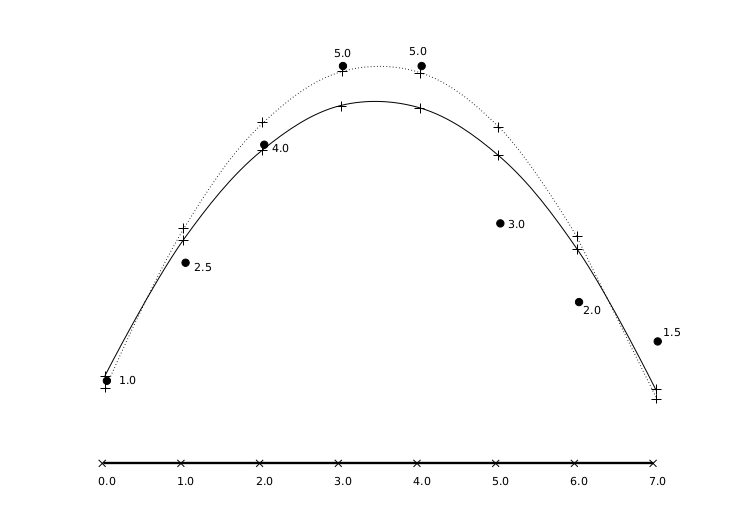
\includegraphics[width=\textwidth]{figures/GLS.png}
	\end{center}
	\caption{Global Least Squares (solid curve) and Weighted Global Least Squares (dashed curve) fit for data represented by the solid circles. The fit is a quadratic fit. The weighting used for the dashed curve is 1.0 every where except at x = 3.0 and x = 4.0 where it is 10.0 (\cite{MLSIntro})}
	\label{fig:gls_example}
\end{figure}
\subsection{Weighted GLS}
\subsection{Weighted Local Least Squares}
\subsection{Mooving Least Squares}

\section{Algorithm}
\subsection{Kernel size and offset}
\subsection{MLS neighborhood search}
\subsection{Similarity threshold}
\section{Results}
\section{Performance analysis}
\section{Conclusions}